% Mathematical extension draft, not yet included by paper.tex.
% The scalar classification is Lean-verified. The unrestricted matrix reduction
% below is a conventional proof under review; see PAPER_CONTEXT.md.
\section{Exact Schatten costs for complex subspace transport}
\label{sec:schatten-optimization}

Fix $1<p<2$. For $0\leq t\leq\pi$, set
\[
 f_p(t)=\bigl(2\sin(t/2)\bigr)^p,
 \qquad
 a_p(t)=\cos(t/2)\bigl(2\sin(t/2)\bigr)^{p-1},
 \qquad
 \vartheta_p=\arccos\frac{2-p}{p}.
\]
Thus $f_p'=p a_p$ on $(0,\pi)$ and $0<\vartheta_p<\pi/2$.
For a principal angle $\theta\in[0,\pi/2]$, define
\begin{equation}
 m_p(\theta)=\min_{0\leq\delta\leq\theta}
       \{f_p(\theta+\delta)+f_p(\theta-\delta)\}.
 \label{eq:schatten-plane-cost}
\end{equation}
Multiplying a planar direct rotation by $e^{i\delta}$ changes its two
eigenphases from $(\theta,-\theta)$ to $(\theta+\delta,-\theta+\delta)$.
The expression in \cref{eq:schatten-plane-cost} is its full displacement
Schatten power sum.

Bolotnikov, Li, and Rodman \citep[Lemmas~3.2--3.3]{bolotnikov2001minimal}
solve the planar problem for $p\geq2$ and the right-angle case for
$1\leq p<2$. Their general constrained problem also includes subspace
transport. The following scalar classification supplies the dependence on
the angle in the remaining exponent range.

\begin{proposition}[The scalar phase diagram]
\label{prop:schatten-scalar-diagram}
The minimum in \cref{eq:schatten-plane-cost} has the following description.
\begin{enumerate}
 \item If $0\leq\theta\leq\vartheta_p$, its unique minimizing phase is
 $\delta=0$, and $m_p(\theta)=2f_p(\theta)$. Its phase derivative is
 strictly positive on $(0,\theta)$.
 \item If $\vartheta_p<\theta<\pi/2$, its unique minimizing phase
 $\delta_p(\theta)$ is the unique solution in $(0,\theta)$ of
 \begin{equation}
    a_p(\theta+\delta)=a_p(\theta-\delta).
    \label{eq:schatten-stationary-balance}
 \end{equation}
 \item At $\theta=\pi/2$, the unique minimizing phase is $\delta=\theta$,
 and $m_p(\pi/2)=2^p$.
\end{enumerate}
\end{proposition}

\begin{proof}
For $0\leq\delta<\theta<\pi/2$, both amplitudes in
\cref{eq:schatten-stationary-balance} are positive. Their logarithmic ratio
\[
 D_{p,\theta}(\delta)=
       \log a_p(\theta+\delta)-\log a_p(\theta-\delta)
\]
has the same sign as the derivative of the objective in
\cref{eq:schatten-plane-cost}. Direct differentiation gives
\begin{equation}
 D_{p,\theta}'(\delta)=
 \frac{\sin\theta\,[p\cos\theta-(2-p)\cos\delta]}
      {\cos^2\delta-\cos^2\theta}.
 \label{eq:schatten-log-ratio-derivative}
\end{equation}
The denominator is positive on $(0,\theta)$, and the bracket in the
numerator increases strictly there. If $\theta\leq\vartheta_p$, that
bracket is positive for every $\delta>0$, including when it vanishes at
$\delta=0$. Since $D_{p,\theta}(0)=0$, the objective increases strictly
on $[0,\theta]$.

If $\theta>\vartheta_p$, the bracket starts negative and ends positive.
Consequently $D_{p,\theta}$ first decreases and then increases. Moreover,
$D_{p,\theta}(\delta)\to+\infty$ as $\delta\uparrow\theta$, because
$a_p(2\theta)>0$ and $a_p(0)=0$. It has exactly one positive zero, and
the objective decreases before that zero and increases afterward.
Continuity includes the endpoint $\delta=\theta$.

For $\theta=\pi/2$, \cref{eq:schatten-log-ratio-derivative} becomes
$D_{p,\pi/2}'(\delta)=-(2-p)/\cos\delta<0$. The objective therefore
decreases strictly up to its endpoint, where its two displacement singular
values are $2$ and $0$. The case $\theta=0$ has only one admissible phase.
\end{proof}

\begin{figure}[t]
 \centering
 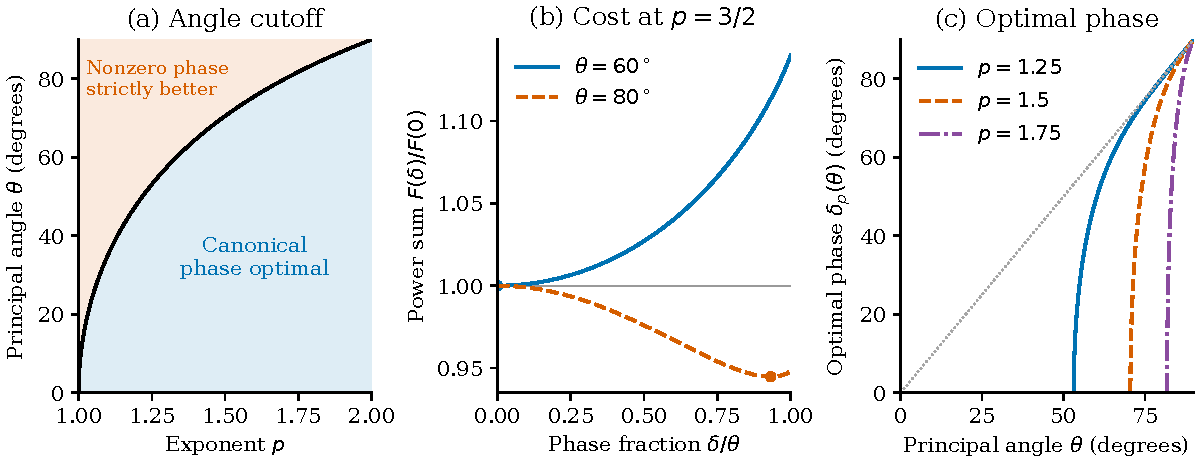
\includegraphics[width=\linewidth]{figures/schatten_phase_diagram.pdf}
 \caption{The scalar phase transition. The cutoff is
 $\vartheta_p=\arccos((2-p)/p)$. At $p=3/2$, the canonical phase minimizes
 the cost at $60^\circ$, while an interior phase gives a smaller cost at
 $80^\circ$. The optimizing phase starts at zero and approaches the
 principal angle at the right-angle boundary.}
 \label{fig:schatten-phase-diagram}
\end{figure}

The scalar minimization determines the unrestricted complex problem as well.
Write $\mathcal U(P,Q)=\{W\in U(n):WPW^*=Q\}$ for the transporters of
two orthogonal projections of equal rank.

\begin{theorem}[Independent principal-plane minimization]
\label{thm:schatten-independent-planes}
Let $P,Q$ be orthogonal projections of rank $r$ on $\mathbb C^n$, and let
$\theta_1,\ldots,\theta_r\in[0,\pi/2]$ be their principal angles, with
multiplicity. Then
\begin{equation}
 \boxed{\min_{W\in\mathcal U(P,Q)}\|I-W\|_p^p
                 =\sum_{j=1}^r m_p(\theta_j).}
 \label{eq:schatten-unrestricted-minimum}
\end{equation}
An attaining transporter is the identity on the fixed summands of a
cosine--sine decomposition and, on each nonzero principal plane, a scalar
phase of the direct rotation with phase $\delta_p(\theta_j)$ or its
negative. In particular, allowing transports that mix principal planes
cannot lower the minimum.
\end{theorem}

We give the reduction to principal planes before proving the theorem.
Extend the scalar cost to the $2\pi$-periodic function
\[
 \phi_p(t)=\bigl(2|\sin(t/2)|\bigr)^p.
\]
It is continuously differentiable because $p>1$. If
$W=\sum_j e^{it_j}E_j$ is a spectral decomposition of a unitary, put
\[
 G_p(W)=\sum_j\phi_p'(t_j)E_j.
\]
The definition is independent of the phase representatives. This
self-adjoint operator commutes with $W$.

\begin{proposition}[First variation and two spectral roots]
\label{prop:schatten-critical-blocks}
If $W$ is a local minimum of the displacement power on $\mathcal U(P,Q)$ and
$J=2P-I$, then
\begin{equation}
 JG_p(W)J=-G_p(W).
 \label{eq:schatten-gradient-anticommutation}
\end{equation}
For each positive eigenvalue $g$ of $G_p(W)$, the spaces $H_g$ and
$H_{-g}$ have the same dimension. Identifying them by $J$, the restriction
of $W$ to their sum has the form
\begin{equation}
 W_+=e^{ia}\exp\bigl(i(b-a)A\bigr),\qquad
 W_-=e^{-ia}\exp\bigl(-i(b-a)B\bigr),
 \label{eq:schatten-critical-two-roots}
\end{equation}
where $A,B$ are orthogonal projections on $H_g$ and
\[
 0<a<\vartheta_p<b<\pi,\qquad p a_p(a)=p a_p(b)=g.
\]
When $g=p a_p(\vartheta_p)$, both restrictions instead have the single
eigenphase $\vartheta_p$ and $-\vartheta_p$, respectively.
\end{proposition}

\begin{proof}
For a Hermitian $H$ commuting with $P$, the curve $W\exp(itH)$ remains
in $\mathcal U(P,Q)$. The spectral first-derivative formula gives
\begin{equation}
 \left.\frac{d}{dt}\|I-W\exp(itH)\|_p^p\right|_{t=0}
              =\operatorname{tr}(G_p(W)H).
 \label{eq:schatten-first-variation}
\end{equation}
For completeness, choose a local logarithm of the unitary near $W$ with
its cut outside the finite spectrum. Apply the differentiability theorem
for Hermitian spectral functions \citep[Theorem~1.1]{lewis1996derivatives}
to the resulting Hermitian logarithm. In an eigenbasis, differentiating
$W\exp(itH)$ shows that the diagonal entries of the logarithm's derivative
are those of $H$, which gives \cref{eq:schatten-first-variation}.
The derivative vanishes for every such $H$. Taking $H$ supported on
either diagonal block relative to $P\oplus P^\perp$ shows that the two
diagonal compressions of $G_p(W)$ vanish. This is
\cref{eq:schatten-gradient-anticommutation}.

The operator $J$ therefore interchanges $H_g$ and $H_{-g}$. On their sum
we can write $J=\left(\begin{smallmatrix}0&I\\I&0\end{smallmatrix}\right)$.
Since $W$ commutes with $G_p(W)$, it is block diagonal there. On
$(0,\pi)$,
\begin{equation}
 a_p'(t)=\frac12\bigl(2\sin(t/2)\bigr)^{p-2}
                    [p\cos t-(2-p)].
 \label{eq:schatten-amplitude-derivative}
\end{equation}
Thus $a_p$ increases strictly up to $\vartheta_p$ and decreases strictly
afterward, with zero endpoint values. The equation $p a_p(t)=g$ has
exactly the two stated roots, except at its maximum, where the roots
coincide. The signs of $\phi_p'$ distinguish the positive and negative
phase spaces and give \cref{eq:schatten-critical-two-roots}.
\end{proof}

\begin{proposition}[Exclusion of overlapping large-phase spaces]
\label{prop:schatten-no-mixing}
At a local minimum, the two large-phase projections in
\cref{eq:schatten-critical-two-roots} satisfy $AB=0$.
\end{proposition}

\begin{proof}
Suppose $AB\ne0$. The decomposition of a pair of orthogonal projections
\citep{halmos1969two} gives either a common range vector, or a common
two-dimensional reducing space on which
\[
 A=\begin{pmatrix}1&0\\0&0\end{pmatrix},\qquad
 B=\begin{pmatrix}c^2&cs\\cs&s^2\end{pmatrix},
 \qquad c=\cos\gamma>0,\quad s=\sin\gamma>0,
 \quad 0<\gamma<\pi/2.
\]
On that space set
\begin{equation}
 X=\begin{pmatrix}2c&s\\s&0\end{pmatrix}.
 \label{eq:schatten-mixing-direction}
\end{equation}
The compressions of $X$ to both small-phase spaces vanish:
\[
 (I-A)X(I-A)=(I-B)X(I-B)=0,
 \qquad AXA=2cA,\quad BXB=2cB.
\]
Extend $X$ by zero and use the same $X$ on $H_g$ and $H_{-g}$. The
resulting Hermitian $H=\operatorname{diag}(X,X)$ commutes with $J$, so
$W\exp(itH)$ is a feasible curve.

The second variation on this four-dimensional block can be computed from
simple eigenphases. For a two-dimensional unitary with distinct phases
$\alpha,\beta$, the phase derivatives under right multiplication by
$\exp(itX)$ are the diagonal entries of $X$ in the eigenbasis. The sum
of the phases is affine in $t$, because its exponential is the
determinant. If $\phi_p'(\alpha)=\phi_p'(\beta)$, their second-derivative
terms in the cost therefore cancel. The remaining terms are
\[
 \phi_p''(\alpha)X_{\alpha\alpha}^2+
 \phi_p''(\beta)X_{\beta\beta}^2.
\]
Apply this to $W_+$ and $W_-$ separately. The small-phase diagonal
entries are zero and the large-phase entries are $2c$. Hence
\begin{equation}
 \left.\frac{d^2}{dt^2}\|I-W\exp(itH)\|_p^p\right|_{t=0}
                    =8c^2 f_p''(b)<0,
 \label{eq:schatten-mixing-negative-curvature}
\end{equation}
where strict negativity follows from $b>\vartheta_p$ and
\cref{eq:schatten-amplitude-derivative}. This contradicts minimality.
All other spectral blocks stay fixed along the curve, so their possible
zero displacement singular values do not enter this second derivative.

If $A$ and $B$ instead have a common range vector, take $X$ to be its
rank-one projection. The same calculation gives $2f_p''(b)<0$.
Both possibilities are excluded, proving $AB=0$.
\end{proof}

\begin{proof}[Proof of \cref{thm:schatten-independent-planes}]
The feasible set is nonempty and compact, so a minimum exists. Choose a
minimizer $W$ and decompose by the eigenspaces of $G_p(W)^2$. These
spaces reduce $P$, $W$, and $Q=WPW^*$.

Consider a nonzero spectral block. When the amplitude roots coincide,
it is a sum of canonical planes with angle $\vartheta_p$. Otherwise,
\cref{prop:schatten-no-mixing} gives the orthogonal decomposition
\[
 H_g=\operatorname{ran}A\oplus\operatorname{ran}B
              \oplus(\ker A\cap\ker B).
\]
The common kernel produces canonical planes of angle $a$, each with
cost $2f_p(a)=m_p(a)$. Each of the other two summands produces a plane
with eigenphases $(b,-a)$ or $(a,-b)$.

Put $\sigma=(a+b)/2$. We have $a+b<\pi$: indeed,
\[
 \frac{a_p(\pi-a)}{a_p(a)}
        =\tan(a/2)^{2-p}<1,
\]
and $a_p$ decreases strictly on $(\vartheta_p,\pi)$. The phase
$(b-a)/2$ satisfies \cref{eq:schatten-stationary-balance} for
$\theta=\sigma$, so \cref{prop:schatten-scalar-diagram} implies
$\sigma>\vartheta_p$ and $f_p(a)+f_p(b)=m_p(\sigma)$.
To identify the geometric angle, note that on $H_g\oplus H_{-g}$,
\[
 (2Q-I)(2P-I)=
 \operatorname{diag}(W_+W_-^*,W_-W_+^*).
\]
Its scalar phases on the displayed summands are $\pm2a$ or
$\pm(a+b)$, so their principal angles are exactly $a$ or $\sigma$.
The cost on every nonzero spectral block is consequently the sum of
the corresponding $m_p$ costs.

On $\ker G_p(W)$ the unitary has only eigenvalues $1$ and $-1$.
Write $q=\operatorname{rank}(I-W)$ on this block. Its displacement
power sum is $2^p q$. Also
\[
 P-Q=(I-W)P+WP(I-W^*)
 \quad\Longrightarrow\quad
 \operatorname{rank}(P-Q)\leq2q.
\]
The number of positive principal angles on this block is
$\operatorname{rank}(P-Q)/2$, and each has
$m_p(\theta)\leq f_p(2\theta)\leq2^p$. The block's cost is therefore
at least the sum of its principal-plane costs. Combining the blocks
gives the lower inequality in \cref{eq:schatten-unrestricted-minimum}.

For the reverse inequality, use a cosine--sine decomposition of $P,Q$.
On each nonzero principal plane choose the scalar phase from
\cref{prop:schatten-scalar-diagram}, and use the identity on the remaining
fixed space. The orthogonal sum is an admissible unitary. Schatten
power sums add across these blocks, giving exactly the right-hand side
of \cref{eq:schatten-unrestricted-minimum}.
\end{proof}

\begin{proposition}[No nonglobal local minima]
\label{prop:schatten-local-is-global}
Every local minimum of $W\mapsto\|I-W\|_p^p$ on $\mathcal U(P,Q)$
is a global minimum.
\end{proposition}

\begin{proof}
The first-variation decomposition and the exclusion of overlapping
large-phase spaces use only local minimality. As in the theorem's proof,
each nonzero block of $G_p(W)^2$ therefore attains the sum of its scalar
principal-plane minima. It remains to consider $\ker G_p(W)$, where
$W=I-2S$ for an orthogonal projection $S$.

Apply the decomposition of two projections to $P,S$ on this space. A
common one-dimensional reducing space on which $S=1$ cannot occur at a
local minimum: changing the phase $\pi$ toward a smaller angle, while
fixing every other direction, preserves transport and decreases the
cost. On a nontrivial two-dimensional reducing space write
\[
 P=\begin{pmatrix}1&0\\0&0\end{pmatrix},\qquad
 S=\begin{pmatrix}c^2&cs\\cs&s^2\end{pmatrix},\qquad
 c=\cos\gamma,\quad s=\sin\gamma,\quad 0<\gamma<\pi/2.
\]
Set $H=\operatorname{diag}(c^2,-s^2)$ on this block and zero elsewhere.
It commutes with $P$, so $W\exp(itH)$ is feasible. The eigenphases
near $\pi$ and zero are smooth, since these eigenvalues are distinct.
Their first derivatives are, respectively, $c^2-s^2$ and zero. If
$\gamma\ne\pi/4$, the large phase contributes
\[
 2^p-\tfrac12p\,2^{p-2}\cos^2(2\gamma)t^2+o(t^2).
\]
The small phase is $O(t^2)$, so its cost is $O(|t|^{2p})=o(t^2)$.
Thus the total cost decreases for small nonzero $t$, contradicting
local minimality. This argument does not require twice differentiability
of the full objective at a zero displacement singular value.

Every remaining nontrivial block has $\gamma=\pi/4$. There $W$ transports
the line of $P$ to its orthogonal complement, with cost $2^p=m_p(\pi/2)$.
On all remaining fixed directions $W=I$. Consequently the zero-gradient
block also attains exactly its scalar principal-plane cost. Summing the
blocks proves that $W$ attains \cref{eq:schatten-unrestricted-minimum}.
\end{proof}

\begin{corollary}[The sharp exponent-dependent angle cutoff]
\label{cor:schatten-canonical-cutoff}
For an acute complex pair with largest principal angle $\alpha$ (taken
to be zero when the principal-angle list is empty), the
canonical direct rotation minimizes the Schatten displacement if and
only if $\alpha\leq\vartheta_p$. The same inequality is sufficient over
the real field. It is the largest cutoff that works uniformly over
real dimensions: whenever $\vartheta_p<\theta<\pi/2$, a real pair with
two principal angles equal to $\theta$ has a strictly cheaper
orientation-preserving transport.
\end{corollary}

\begin{proof}
The complex assertion follows by summing
\cref{prop:schatten-scalar-diagram}. A real transporter is a complex
transporter after complexification, with unchanged singular values, so
the sufficient condition also holds over the real field. For sharpness,
realify a complex planar scalar-phase improvement. Every displacement
singular value is then repeated twice, both real principal angles are
$\theta$, and the real determinant is the squared modulus of the complex
determinant, hence one.
\end{proof}

\begin{corollary}[A sharp Schatten comparison constant]
\label{cor:schatten-sharp-ratio}
For a principal-plane direct rotation $R$ of a finite-dimensional real
or complex pair, and every admissible transporter $W$,
\begin{equation}
 \|I-R\|_p\leq 2^{1/p-1/2}\|I-W\|_p.
 \label{eq:schatten-sharp-ratio}
\end{equation}
The constant is attained by a right-angle plane in either field and is
the optimal uniform constant for acute pairs as well.
\end{corollary}

\begin{proof}
For a scalar-phase plane, put
$x=2\sin((\theta+\delta)/2)$ and
$y=2\sin((\theta-\delta)/2)$. Then
\[
 x^p+y^p\geq(x^2+y^2)^{p/2}
 \geq\bigl(2(2\sin(\theta/2))^2\bigr)^{p/2},
\]
because $x^2+y^2=4-4\cos\theta\cos\delta
\geq4-4\cos\theta$. Consequently
$2f_p(\theta)\leq2^{1-p/2}m_p(\theta)$.
Sum this inequality and apply \cref{thm:schatten-independent-planes}.
Complexification gives the real inequality. At a right angle the direct
rotation has displacement singular values $(\sqrt2,\sqrt2)$, while a
reflection has $(2,0)$. Their norm ratio is $2^{1/p-1/2}$. Real
reflections on planes with angles tending to $\pi/2$ show that the same
constant is necessary for acute pairs.
\end{proof}

\subsection{Computing the optimizer and resolving the transition}

In the supercritical regime define
\[
 \eta_p(\theta)=\arccos\frac{p\cos\theta}{2-p}.
\]
Equation~\eqref{eq:schatten-log-ratio-derivative} shows that
$D_{p,\theta}$ increases strictly on
$(\eta_p(\theta),\theta)$ and that its unique positive zero lies in
this interval. Bisection of this scalar equation therefore computes the
global plane optimizer with a certified choice of branch. Together with
\cref{thm:schatten-independent-planes}, this reduces the matrix problem
to a cosine--sine decomposition and one scalar root for each supercritical
principal angle.

At $p=3/2$ that root is explicit. Writing $c=\cos\theta$, one obtains
\begin{equation}
 \delta_{3/2}(\theta)=\arccos\frac{c}{1-2c},\qquad
       \arccos(1/3)<\theta\leq\pi/2,
 \label{eq:schatten-three-halves-phase}
\end{equation}
and
\begin{equation}
 m_{3/2}(\theta)^{2/3}=
 \begin{cases}
  2^{2/3}\,2\sin(\theta/2),&0\leq\theta\leq\arccos(1/3),\\
  2(1+c)^{1/3}(1-2c)^{1/6},&\arccos(1/3)\leq\theta\leq\pi/2.
 \end{cases}
 \label{eq:schatten-three-halves-value}
\end{equation}
To verify these formulas above the transition, put
$x=2\sin((\theta+\delta)/2)$ and
$y=2\sin((\theta-\delta)/2)$. Squaring the positive stationary
amplitudes gives $x-x^3/4=y-y^3/4$. Since $x>y$, this is equivalent to
$x^2+xy+y^2=4$. The identities
\[
 x^2+y^2=4-4c\cos\delta,\qquad
 xy=2(\cos\delta-c)
\]
give $(1-2c)\cos\delta=c$ and hence
\cref{eq:schatten-three-halves-phase}. Moreover,
\[
 x+y=\frac{2(1-c)}{\sqrt{1-2c}},\qquad
 \sqrt{xy}=\frac{2c}{\sqrt{1-2c}}.
\]
Using $x^{3/2}+y^{3/2}
=\sqrt{x+y+2\sqrt{xy}}\,(x+y-\sqrt{xy})$ proves
\cref{eq:schatten-three-halves-value}. Continuity includes the two
displayed boundary angles.

The transition also determines the smoothness of the minimum value.
Fix $p$ and write $c_p=2\sin(\vartheta_p/2)$ and
$\varepsilon=2-p-p\cos\theta$. Expanding the logarithmic ratio at
$(\vartheta_p,0)$ gives
\[
 D_{p,\theta}(\delta)
 =\frac{\delta}{\sin\vartheta_p}
   \left[-\varepsilon+\frac{2-p}{6}\delta^2
       +O(\varepsilon^2+\varepsilon\delta^2+\delta^4)\right].
\]
The implicit function theorem applied after dividing by $\delta$ and
using $\delta^2$ as the variable yields
\begin{equation}
 \delta_p(\theta)^2
    =\frac{6\varepsilon}{2-p}+O(\varepsilon^2),\qquad
 m_p(\theta)=2f_p(\theta)
    -\frac{3p c_p^{p-2}}{2(2-p)}\varepsilon^2
    +O(\varepsilon^3),
 \label{eq:schatten-transition-asymptotics}
\end{equation}
as $\theta\downarrow\vartheta_p$ from above. In particular, the
nonzero optimizing phase grows as the square root of the excess angle.
The minimum value is continuously differentiable at the transition, but
its one-sided second derivatives are
\[
 m_p''(\vartheta_p-)=0,\qquad
 m_p''(\vartheta_p+)
   =-\frac{3p^3 c_p^{p-2}\sin^2\vartheta_p}{2-p}<0.
\]
Thus the quotient displacement cost loses twice differentiability at an
acute angle determined by $p$, before the geometric right-angle boundary.

\subsection{Schatten-class perturbations in a Hilbert space}

The finite-dimensional formula also gives an attained minimum in the
Schatten ideal. Let $\mathcal S_p$ denote the Schatten class on a separable
complex Hilbert space $\mathcal H$.

\begin{theorem}[An optimum differing by finite rank from direct rotation]
\label{thm:schatten-ideal-minimum}
Let $P,Q$ be orthogonal projections with $P-Q\in\mathcal S_p$ and
\[
 \dim(\operatorname{ran}P\cap\ker Q)
   =\dim(\ker P\cap\operatorname{ran}Q).
\]
List their positive principal angles with multiplicity as
$(\theta_j)_{j\geq1}$, using a finite list when appropriate. Then
\begin{equation}
 \min_{\substack{W\text{ unitary},\ WPW^*=Q\\ I-W\in\mathcal S_p}}
       \|I-W\|_p^p=\sum_j m_p(\theta_j).
 \label{eq:schatten-ideal-minimum}
\end{equation}
For any principal-plane direct rotation $R$, including a choice of pairing
on the right-angle defect spaces, an attaining $W_*$ can be chosen with
\begin{equation}
 \operatorname{rank}(W_*-R)
       \leq 2\,\#\{j:\theta_j>\vartheta_p\}<\infty.
 \label{eq:schatten-finite-correction}
\end{equation}
In particular, $R$ is optimal if and only if all principal angles are at
most $\vartheta_p$.
\end{theorem}

\begin{proof}
The decomposition of two projections \citep{halmos1969two}, together with
compactness of $P-Q$, gives orthogonal principal planes for all nonzero
angles and a fixed complement. The defect-space hypothesis allows the
right-angle spaces to be paired. Since the nonzero singular values of
$P-Q$ are $\sin\theta_j$, each twice, we have
$\sum_j\sin^p\theta_j<\infty$ and $\theta_j\to0$ if the list is infinite.
The direct rotation $R$ is the identity on the fixed complement and has
two displacement singular values $2\sin(\theta_j/2)$ on each plane.
The inequality $2\sin(\theta/2)\leq\sqrt2\sin\theta$ on
$[0,\pi/2]$ implies $I-R\in\mathcal S_p$.

First suppose the angle list is infinite, and let $R_N$ be $R$ on its
first $N$ principal planes and the identity elsewhere. Then
$R_N-R\to0$ in $\mathcal S_p$. For any feasible $W$, put $Z=R^*W$.
It commutes with $P$ and satisfies $Z-I\in\mathcal S_p$. The compact
normal operator $Z-I$ has an orthonormal eigenbasis off its kernel.
Because $Z$ commutes with $P$, its finite-dimensional nontrivial
eigenspaces admit bases in $\operatorname{ran}P$ or $\ker P$.
Truncating these eigenspaces gives unitaries $Z_N$ commuting with $P$,
with $Z_N-I$ of finite rank and $Z_N-Z\to0$ in $\mathcal S_p$.

Set $W_N=R_N Z_N$ and $Q_N=R_N P R_N^*$. The ranges of $R_N-I$ and
$Z_N-I$ lie in a common finite-dimensional $P$-invariant space $M_N$.
Both unitaries preserve $M_N$ and equal the identity on its orthogonal
complement. Their product transports $P|_{M_N}$ to $Q_N|_{M_N}$.
The latter pair has the first $N$ positive principal angles of $P,Q$,
with any remaining angles zero. Thus
\cref{thm:schatten-independent-planes} gives
\[
 \|I-W_N\|_p^p\geq\sum_{j=1}^N m_p(\theta_j).
\]
Unitary invariance and the ideal norm inequality yield
\[
 \|W_N-W\|_p
  \leq\|R_N-R\|_p+\|Z_N-Z\|_p\longrightarrow0.
\]
Passing to the limit proves the lower bound. For a finite angle list,
keep $R_N=R$ and use the same approximation of $Z$.

Choose $W_*$ by the independently minimizing phases on the principal
planes and the identity on the fixed complement. Its cost is the sum
in \cref{eq:schatten-ideal-minimum}, bounded above by the finite cost of
$R$. Only finitely many angles exceed the positive number
$\vartheta_p$. Every other plane uses phase zero, proving
\cref{eq:schatten-finite-correction}. The optimality criterion follows
from the scalar classification and its strict improvement above the
transition.
\end{proof}
